\documentclass{report}
\usepackage{lmodern}
\usepackage[french]{babel}
\usepackage[utf8]{inputenc}
\usepackage{graphicx}
\usepackage{subcaption}
\usepackage{amsmath, amsfonts, amssymb} 

\begin{document}

\section{R\'esolution par la m\'ethode d'Euler implicite}\\

\textbf{Definition des variables et des param\`etres : }
On d\'efinit tout d'abord les diff\'erentes variables dont on a besoin pour d\'ecrire les \'equations du sch\'ema d'Euler implicite : \\
\begin{itemize}
\item On fixe comme param\`etres $a = 0.2$ et $b = 1.3$ pour satisfaire les conditions $(a+b)^3>b-a$} et $b>a$.\\

\item On appelle $N_x$ le nombre d'it\'erations sur la variable d'espace, avec $x$ variant entre 0 et 1, on a donc $dx = \frac{1}{N_x}$. On a pris ici $N_x = 30$.\\

\item On garde la notation $c = \begin{pmatrix} u \\ v \end{pmatrix}$, qui sera de taille $2 N_x$.\\

\item Le pas de temps doit \^etre assez petit, $dt = 10^{-3}$ suffit, en dessous, le sch\'ema diverge. On prend de plus une plage de temps suffisamment grande pour que les modes puissent appara\^itre, par exemple $N_t = 50 000$, voire plus si n\'ecessaire.\\

\item Dans une variable $stock$ (tableau de taille $(2N_x,N_t)$)sont stock\'ees toutes les valeurs de $u$ et $v$.\\
\end{itemize}\\

\textbf{Initialisation autour de la solution d'\'equilibre : }\\
On se place autour de la solution d'\'equilibre, calcul\'ee comme \'etant $u_{eq} = a+b$ et $v_{eq} = \frac{b}{(a+b)^2}$, en ajoutant un nombre al\'eatoire compris entre $-10^{-4}$ et $10^{-4}$.
\begin{figure}[h!]
\center{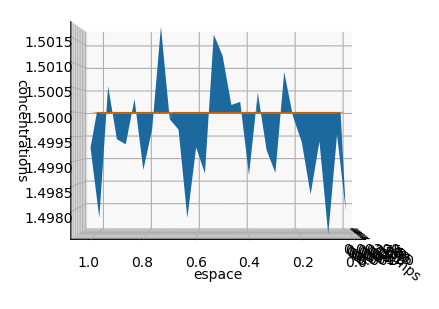
\includegraphics[scale = 0.8]{cond_init.png}}
\caption{Conditions initiales al\'eatoires autour de l'\'equilibre}
\label{fig cond init}
\end{figure}
\\

\textbf{Matrices du Laplacien et de Diffusion :}\\
Nous avons besoin de l'op\'erateur Laplacien discret dont la matrice, de taille  $(N_x, N_x)$, s'\'ecrit  : \\
\begin{displaymath}
Lp = \frac{1}{dx^2} \begin{pmatrix} 
-2     & 1     & 0      & \cdots & 1\\
 1     & -2    & \ddots & \ddots & \vdots\\
 0     &\ddots & \ddots & \ddots & 0\\
\vdots & \ddots& \ddots & \ddots & 1\\
1      &\cdots & 0      &    1   & -2
\end{pmatrix}
\end{displaymath}\\

Ce qui donne, \'ecrite par blocs ($1^{er}$ bloc appliqu\'e \`a $u$, le $2^{nd}$ \`a $v$):\\
\begin{displaymath}
A = \begin{pmatrix} 
Lp  & 0 \\
 0  & Lp
\end{pmatrix}
\end{displaymath}\\

Il nous faut \'egalement la matrice de diffusion, qui s'\'ecrit simplement par blocs, pour un coefficient de diffusion $d$ et en notant $I$ la matrice identit\'e de dimensions $(N_x, N_x)$ :\\
\begin{displaymath}
D = \begin{pmatrix} 
I  & 0 \\
 0  & dI
\end{pmatrix}
\end{displaymath}\\

Si on note $c^n = \begin{pmatrix} u^n \\ v^n \end{pmatrix}$ le vecteur $c$ \`a l'instant $t_n = n dt$, le sch\'ema d'Euler implicite s'\'ecrit :\\
\begin{equation}
c^{n+1} = c^n + dt (DA c^{n+1} + \delta f(c^{n+1}))
\end{equation}\\

On utilise ici un sch\'ema d'Euler simplifi\'e dans le sens o\`u on remplace $f(c^{n+1})$ par simplement $f(c^n)$. On obtient ainsi :\\
\begin{align}
c^{n+1} = c^n + dt (DA c^{n+1} + \delta f(c^n)) \nonumber\\
\nonumber \\
c^{n+1} = (I + dt DA)^{-1} (c^n + dt \delta f(c^n))
\end{align}\\

On it\`ere ainsi ce sch\'ema $N_t$ fois, et \`a chaque it\'eration, on stock le r\'esultat en remplissant la $n^{i\`eme}$ ligne de la matrice $stock$:\\
\begin{equation}
stock(n, 1:2 N_x) = c^n
\end{equation}\\
 
\textbf{R\'esultats : }\\

On se place \`a $d=30$ et $\delta= 120$. Sur le diagramme de Turing, on anticipe la stabilit\'e des deux premiers modes, et on s'attend \`a voir apparap\^itre le mode 2. C'est en effet ce que l'on observe : \\
\begin{figure}[h!]
\center{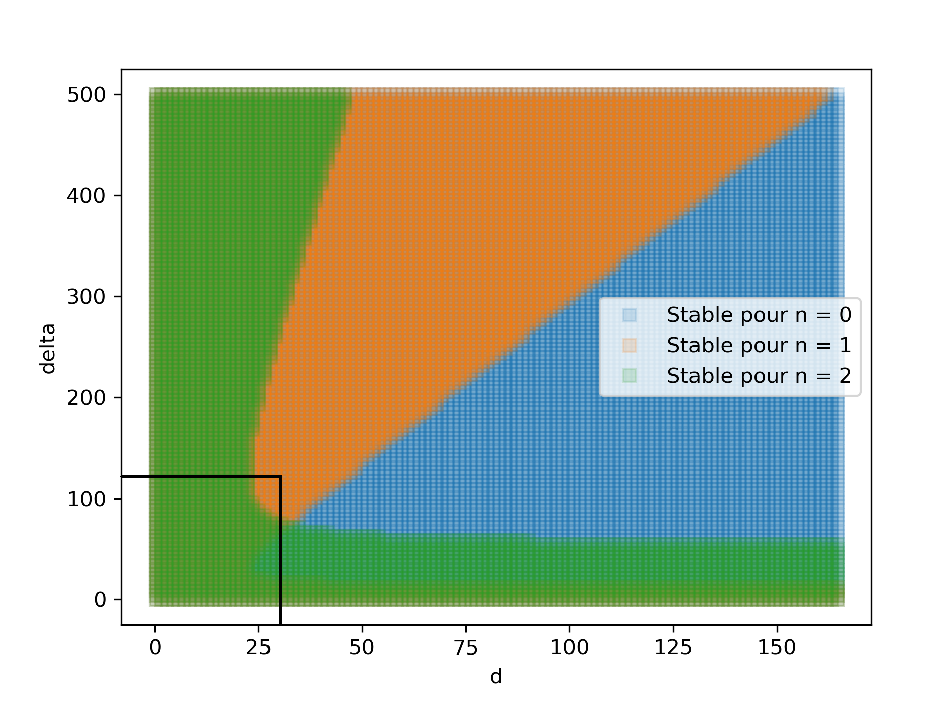
\includegraphics[scale = 0.25]{diagrammes_turing20-120.png}}
\caption{Diagramme de Turing : instabilit\'e du mode 2}
\label{fig turing1}
\end{figure}\\


\begin{figure}[h!]
\center{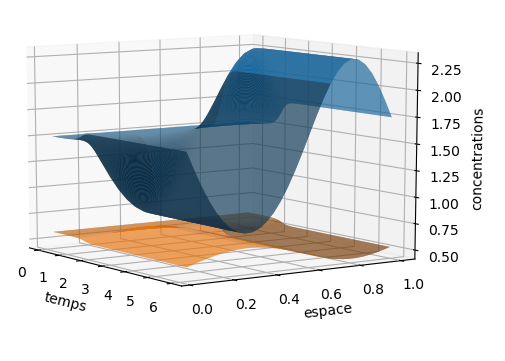
\includegraphics[scale = 0.7]{d30delta120.png}}
\caption{Concentrations u et v pour $d=30$ et $\delta = 120$}
\label{fig concentration1}
\end{figure}\\


On peut examiner d'autres cas, o\`u les modes instables se superposent  : \\

\begin{figure}[h!]
\center{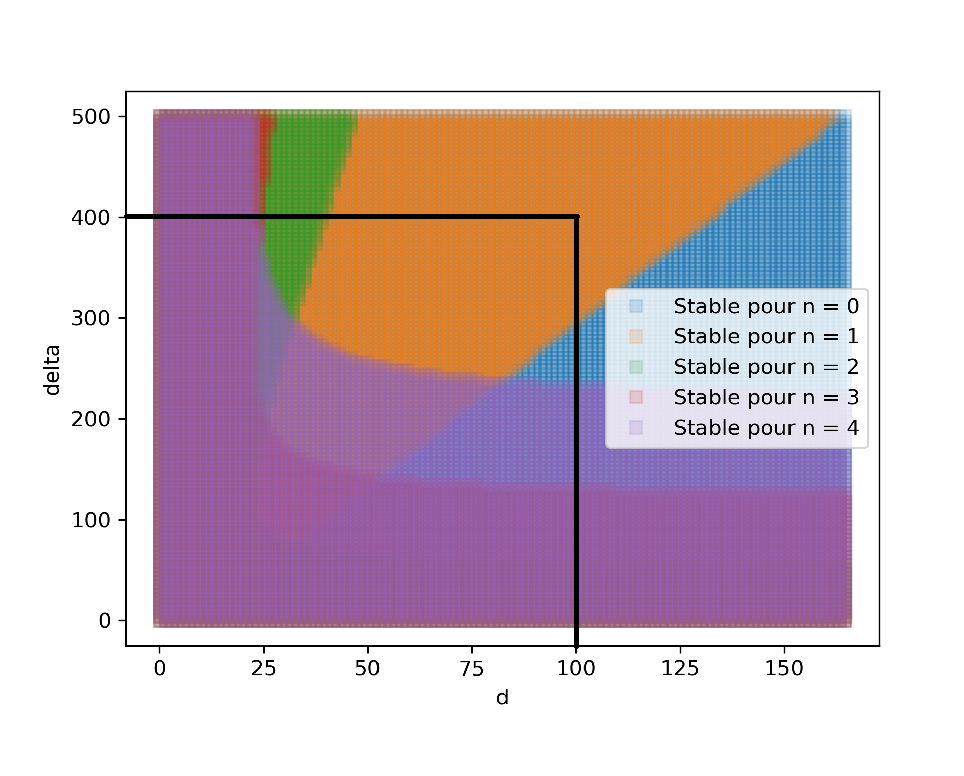
\includegraphics[scale = 0.25]{diagrammes_turing100-400.png}}
\caption{Diagramme de Turing : superposition de modes instables}
\label{fig turing2}
\end{figure}\\

\begin{figure}[h!]
  \centering
  \begin{subfigure}[h]{0.4\linewidth}
    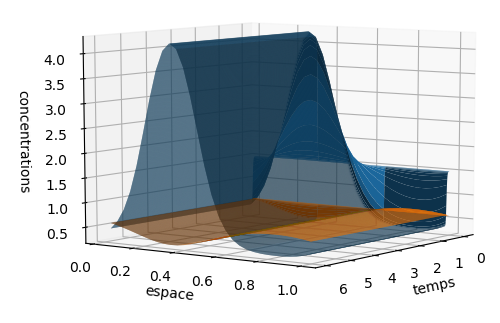
\includegraphics[width=\linewidth]{d100delta400.png}
  \end{subfigure}
  \begin{subfigure}[h]{0.4\linewidth}
    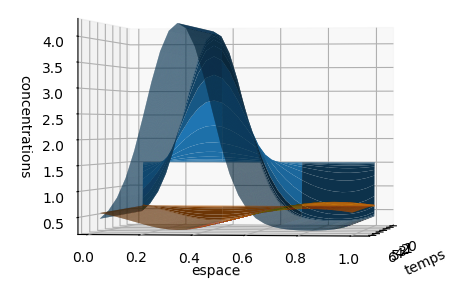
\includegraphics[width=\linewidth]{d100delta400_1.png}
  \end{subfigure}
  \caption{Concentrations pour $d=100$ et $\delta=400$}
  \label{fig concentration2}
\end{figure}


\begin{figure}[h!]
\center{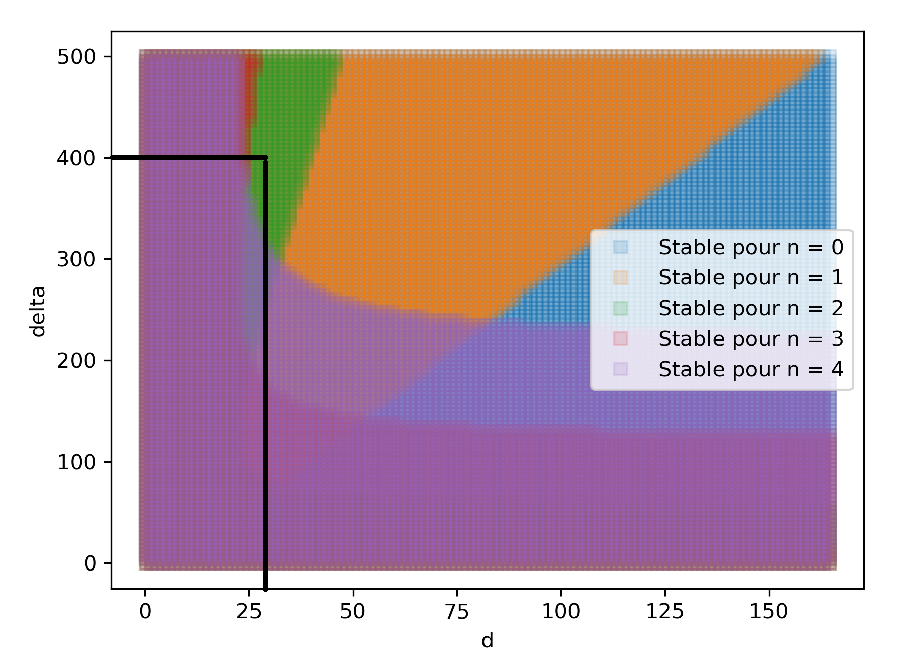
\includegraphics[scale = 0.25]{diagrammes_turing30-400.png}}
\caption{Diagramme de Turing : superposition de modes instables 2}
\label{fig turing3}
\end{figure}\\

\begin{figure}[h!]
  \centering
  \begin{subfigure}[h]{0.4\linewidth}
    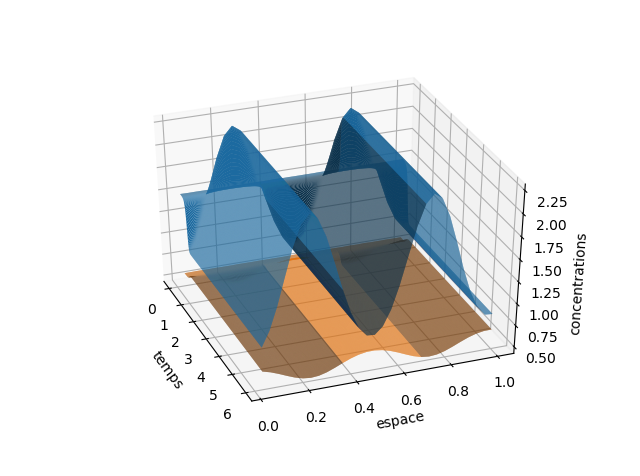
\includegraphics[width=\linewidth]{d30delta450.png}
  \end{subfigure}
  \begin{subfigure}[h]{0.4\linewidth}
    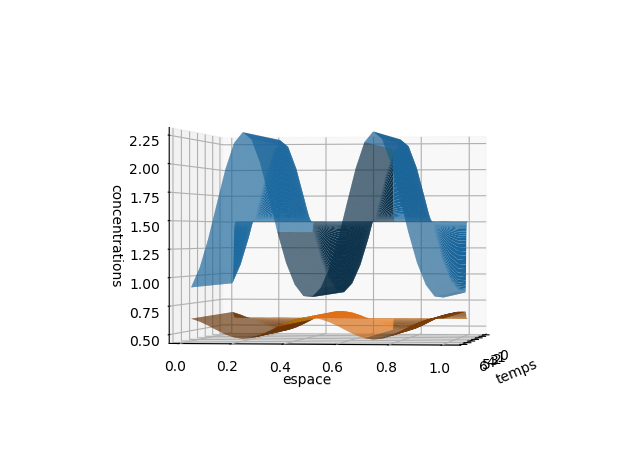
\includegraphics[width=\linewidth]{d30delta400_1.png}
  \end{subfigure}
  \caption{Concentrations pour $d=30$ et $\delta=400$ (mode 3 instable}
  \label{fig concentration3}
\end{figure}


\begin{figure}[h!]
\center{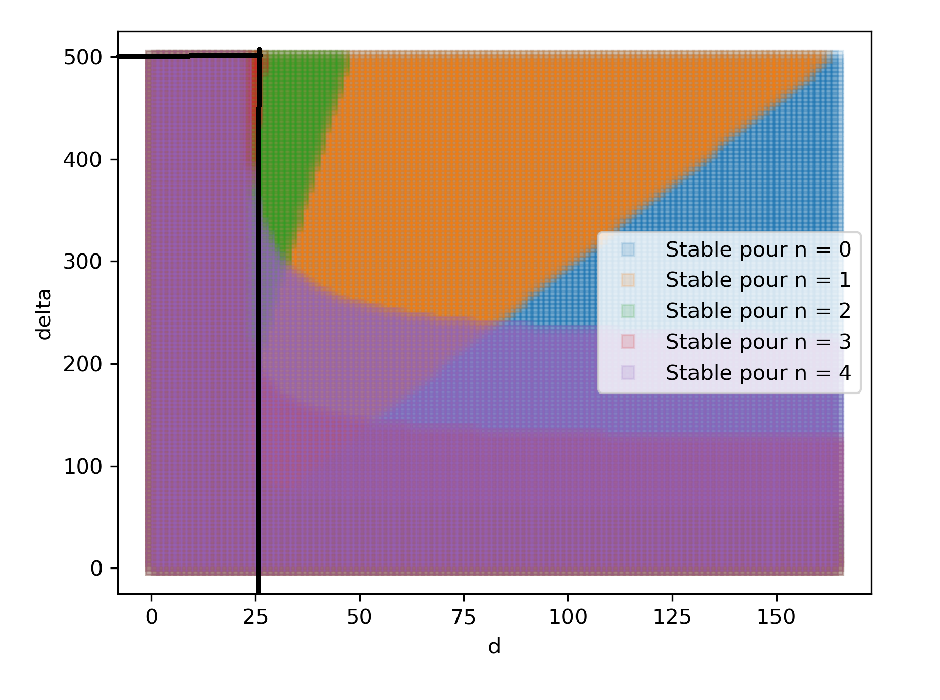
\includegraphics[scale = 0.25]{diagrammes_turing26-500.png}}
\caption{Diagramme de Turing : instabilit\'e du mode 4}
\label{fig turing1}
\end{figure}\\


\begin{figure}[h!]
\center{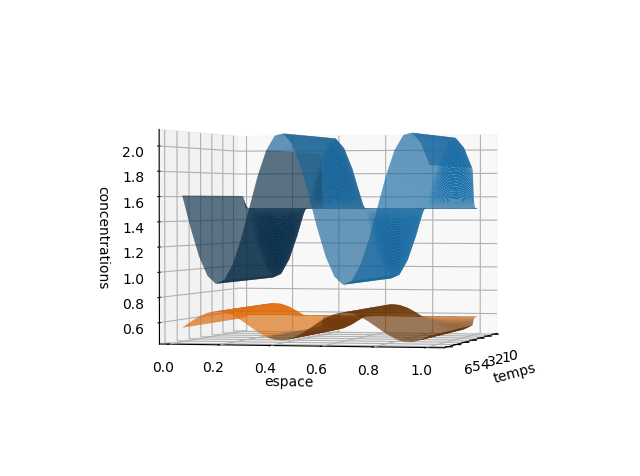
\includegraphics[scale = 0.7]{d26delta500.png}}
\caption{Concentrations u et v pour $d=26$ et $\delta = 500$ (mode 4 instable)}
\label{fig concentration4}
\end{figure}\\

Remarque : plus on est proche du $d_critique$, environ 23, plus les concentrations mettent du temps \`a converger vers une solution ind\'ependante du temps.\\
\begin{figure}[h!]
  \centering
  \begin{subfigure}[h]{0.4\linewidth}
    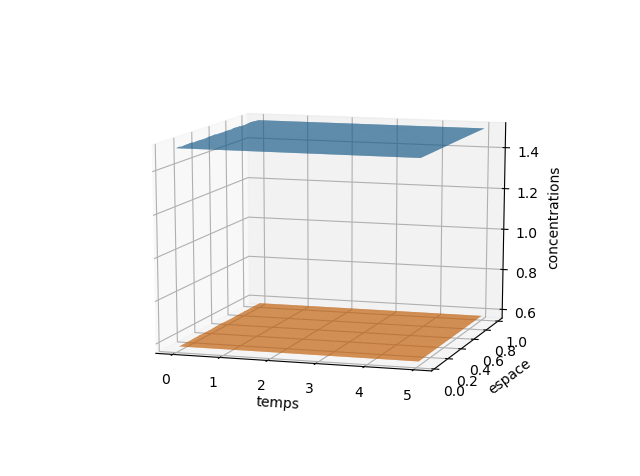
\includegraphics[width=\linewidth]{dcrit5.png}
  \end{subfigure}
  \begin{subfigure}[h]{0.4\linewidth}
    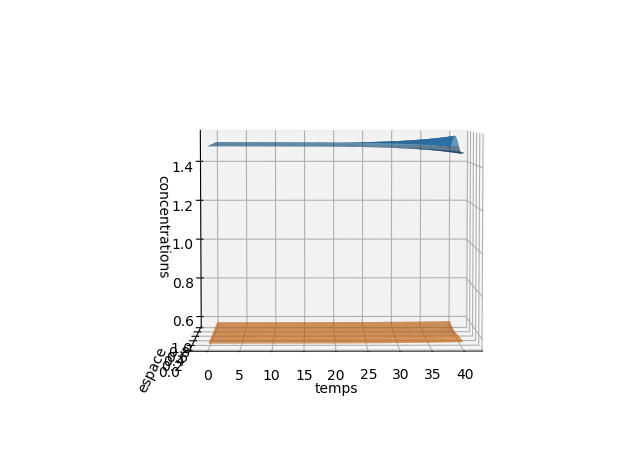
\includegraphics[width=\linewidth]{dcrit40.png}
  \end{subfigure}
	  \begin{subfigure}[h]{0.4\linewidth}
    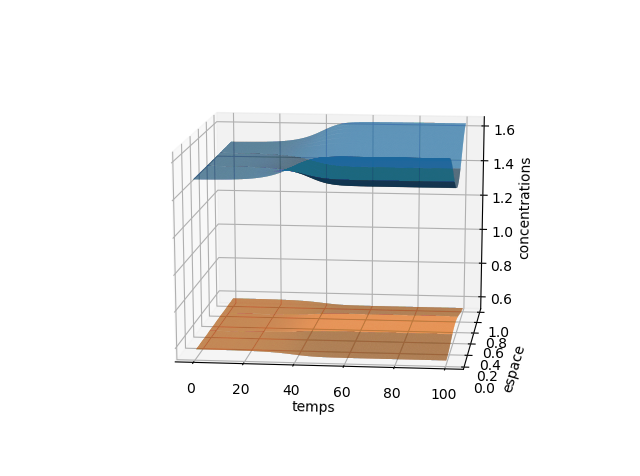
\includegraphics[width=\linewidth]{dcrit100.png}
  \end{subfigure}
  \caption{Concentrations pour $d=23.1$ et $\delta=150$ : convergence apr\`es 50 secondes de temps}
  \label{fig dcrit_tps}
\end{figure}

\end{document}